\documentclass[conference]{IEEEtran}
\usepackage[T1]{fontenc}
\usepackage{lmodern}
\usepackage[utf8]{inputenc}
\usepackage{newtxtext}
\usepackage{tikz}
\usetikzlibrary{positioning,arrows.meta,shapes.multipart,fit,calc,shapes.geometric,shapes,shapes.symbols,arrows}
\usepackage{tabularx}
\usepackage{booktabs}
\usepackage{siunitx}
\sisetup{round-mode=places, round-precision=2}
\usepackage{array}
\usepackage{graphicx}
\usepackage{amsmath}
\usepackage{amssymb}
\usepackage{pifont}
\newcommand{\cmark}{\ding{51}}
\newcommand{\xmark}{\ding{55}}
\usepackage{url}
\usepackage[backend=biber]{biblatex}
\addbibresource{reference.bib}
\addbibresource{demo_refs.bib}
\renewcommand{\textfraction}{0.05}
\renewcommand{\floatpagefraction}{0.8}

\begin{document}

\title{VTTSI-Chat: A Demo of Real-Time Intersection Safety Monitoring\\
with LLM-Powered Natural Language Explanation}

\author{
\IEEEauthorblockN{Jason Cusati}
\IEEEauthorblockA{\textit{Computer Science}\\
Virginia Tech, Blacksburg, VA\\
djjay@vt.edu}
\and
\IEEEauthorblockN{Cheng-Shun Chuang}
\IEEEauthorblockA{\textit{Computer Science}\\
Virginia Tech, Alexandria, VA\\
cchengshun@vt.edu}
\and
\IEEEauthorblockN{Victory Uhunmwangho}
\IEEEauthorblockA{\textit{Computer Science}\\
Virginia Tech, Blacksburg, VA\\
victoryu@vt.edu}
}

\maketitle

\sloppy
\raggedbottom

\begin{abstract}
We demonstrate \textbf{VTTSI-Chat}, an extension of the Virginia Tech Transportation
Safety Index (VTTSI) that adds a Large Language Model (LLM)-powered conversational
interface atop a cloud-native, real-time intersection safety scoring system.
VTTSI fuses Empirical Bayes (EB) crash history with connected-vehicle telemetry
through a hybrid RT--SI and CRITIC-weighted MCDM pipeline, producing an interpretable
0--100 safety score every 15 minutes.
The new SafetyChat module bridges the gap between quantitative safety indices and
human-readable situational awareness: operators, planners, and emergency responders can
ask natural language questions---\emph{``Why is the Glebe--Potomac score elevated?''}
or \emph{``Which intersection carries the highest VRU risk right now?''}---and receive
evidence-grounded, contextual responses generated by a tool-augmented LLM.
Unlike existing traffic-LLM systems focused on signal control or route optimization,
VTTSI-Chat is the first system to pair a hybrid quantitative safety index with
LLM-generated causal safety narratives for transportation management center (TMC) operators.
\end{abstract}

% ─────────────────────────────────────────────────────────
\section{Introduction}
\label{sec:intro}

Real-time intersection safety data are increasingly available through connected-vehicle
infrastructure, yet the gap between a numerical safety score and actionable insight
remains large. Practitioners operating a transportation management center (TMC) must
interpret multi-dimensional indices under time pressure, often without the domain
expertise to distinguish a volume-driven spike from a behavioral anomaly.

Recent large language model (LLM) research demonstrates that tool-augmented models can
reason over structured numerical data and produce accurate, calibrated explanations
\cite{toolformer2023, openai_functioncalling}.
Within transportation, LLM-based efforts have targeted signal control
\cite{llmlight2024} and autonomous vehicle (AV) motion planning
\cite{gptdriver2023,drivevlm2024}, but \emph{safety-index explanation} for
infrastructure operators has not been addressed.

This demo presents \textbf{VTTSI-Chat}, a live system that pairs the existing VTTSI
backend---a hybrid RT--SI + MCDM scoring pipeline deployed on Google Cloud Run---with
a \textbf{SafetyChat} front-end module.
SafetyChat uses a function-calling LLM that queries VTTSI API endpoints, retrieves the
current and historical safety-index components, and constructs grounded natural language
narratives that explain \emph{why} a score is elevated, which signals dominate, and
what operational actions may be warranted.

\textbf{Demo Claim.} VTTSI-Chat is the first system to combine (1) a hybrid
EB-stabilized crash + real-time MCDM safety index with (2) an LLM that explains
safety score components through natural language dialogue for TMC operators.

% ─────────────────────────────────────────────────────────
\section{VTTSI System Overview}
\label{sec:system}

\begin{figure}[t]
    \centering
    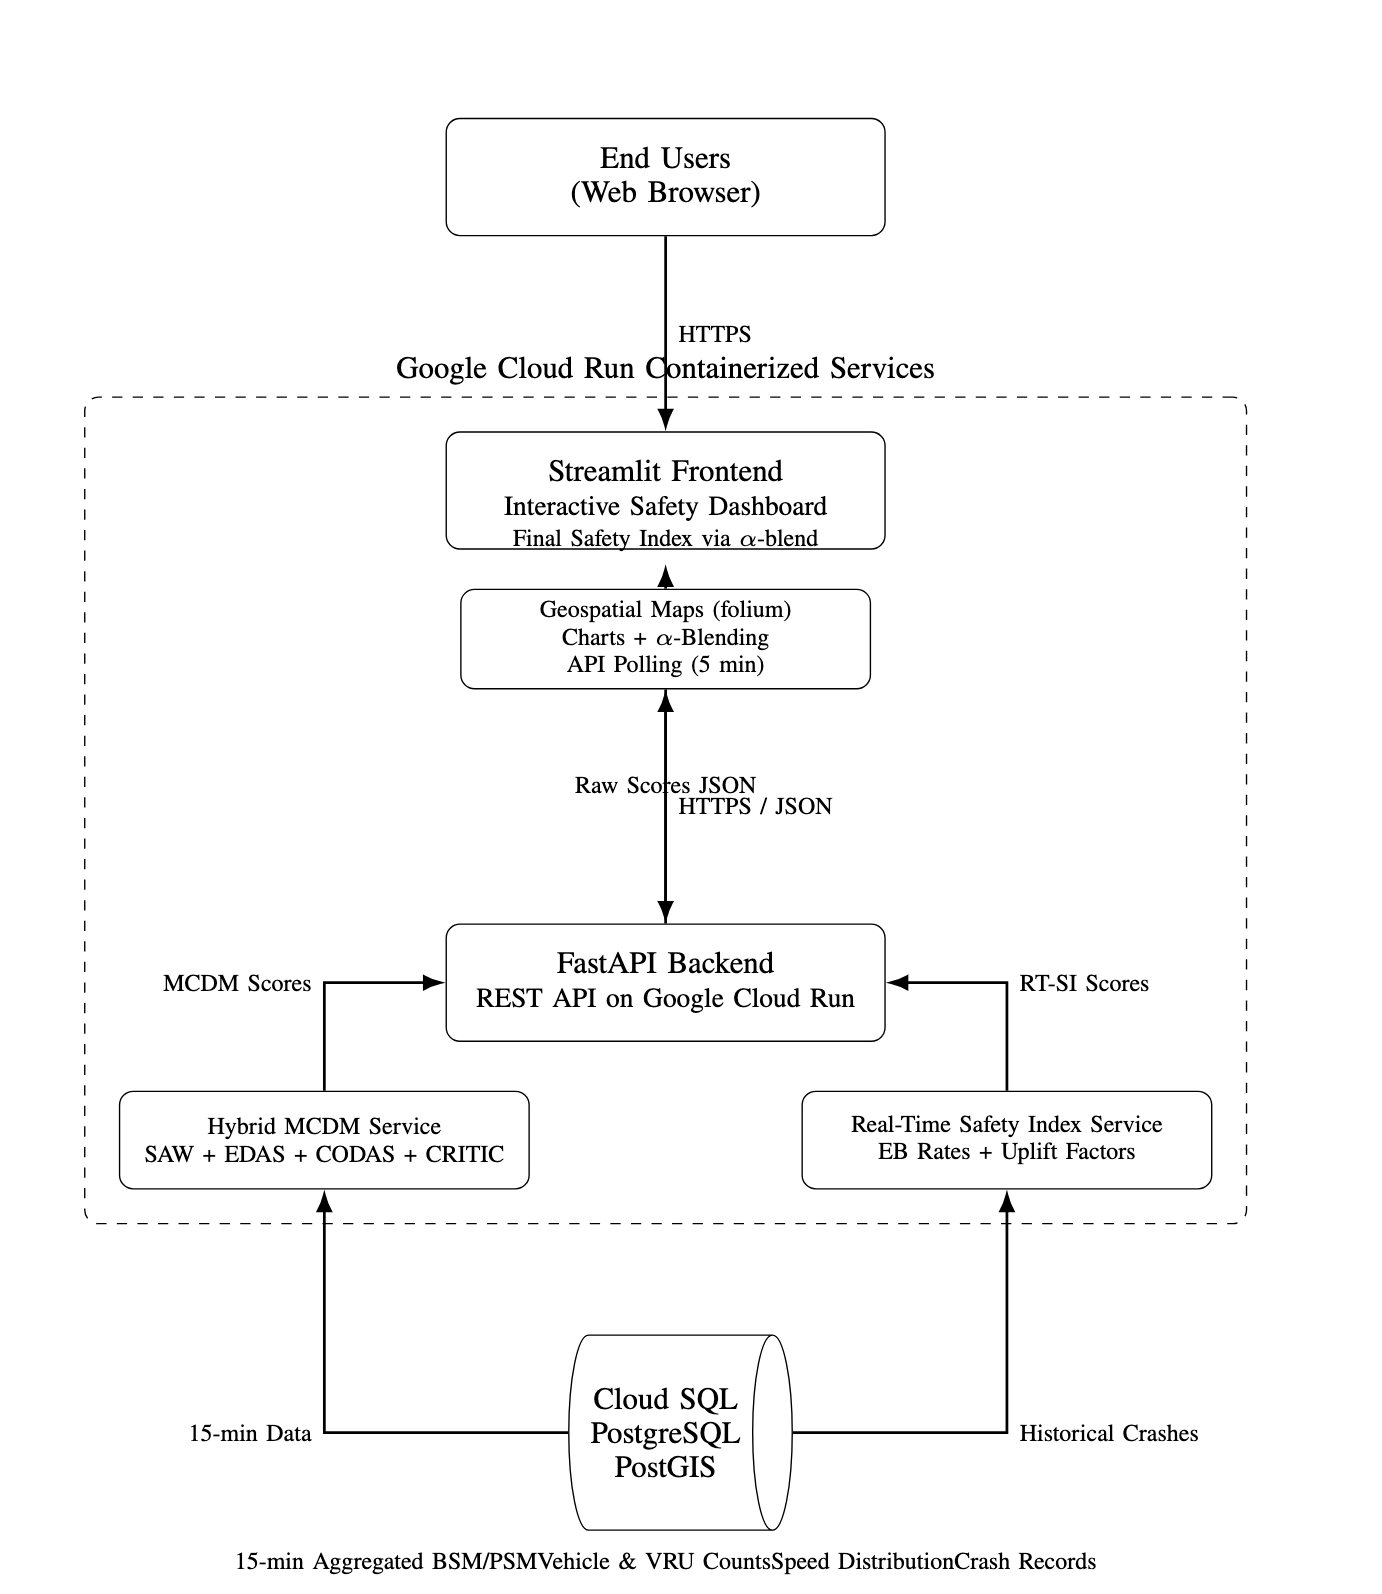
\includegraphics[width=\linewidth]{system-architecture.png}
    \caption{VTTSI cloud architecture extended with the SafetyChat LLM module.
             New components are highlighted with a dashed border.}
    \label{fig:architecture}
\end{figure}

\subsection{Backend Safety Engines}

The VTTSI backend (FastAPI on Google Cloud Run) computes two complementary
safety indices every 15 minutes using data from the VTTI Trino connected-vehicle system.

\textbf{Real-Time Safety Index (RT--SI).}
RT--SI anchors each intersection's risk to a severity-weighted Empirical Bayes baseline
derived from seven years (2017--2024) of VDOT crash records:
\begin{equation}
\hat{r}^{\text{EB}}_{i} = \frac{Y_i + \lambda r_0}{1 + \lambda},
\quad \lambda^\star = 10{,}000,
\end{equation}
and multiplies by bounded real-time uplift factors for speed deficit, speed variance,
and VRU--vehicle conflict exposure.
The resulting $\mathrm{SI}^{\text{RT}} \in [0, 100]$ captures \emph{historically
informed, operationally adjusted} risk.

\textbf{MCDM Safety Index.}
A CRITIC-weighted multi-criteria decision-making pipeline applies SAW, EDAS, and CODAS
over a decision matrix of five real-time criteria (vehicle count, VRU count,
average speed, speed variance, incident count) across 15-minute intersection--time bins.
CRITIC weights are recomputed every 24 hours to adapt to evolving traffic conditions
\cite{Amraji2025CombinedSafetyIndex}.
The hybrid MCDM index $\overline{\mathrm{SI}}^{\mathrm{MCDM}} \in [0, 100]$ captures
\emph{instantaneous operational anomaly}.

\textbf{Blended Final Index.}
\begin{equation}
\mathrm{SI}^{\text{Final}}_{i,t} =
\alpha\,\mathrm{SI}^{\text{RT}}_{i,t} +
(1-\alpha)\,\overline{\mathrm{SI}}^{\text{MCDM}}_{i,t},
\end{equation}
where $\alpha$ is adjustable (default 0.7) to favor either real-time turbulence or
historical risk.

\subsection{Existing Streamlit Dashboard}

The current frontend (Streamlit, Google Cloud Run) provides interactive maps with
intersection risk heat-maps, time-series charts of each index component, correlation
matrices, and the $\alpha$-blending slider. While comprehensive, this dashboard is
passive: it presents data but does not explain what is driving a score or suggest
operator actions.

% ─────────────────────────────────────────────────────────
\section{SafetyChat: LLM-Powered Explanation Module}
\label{sec:safetychat}

\begin{figure}[t]
    \centering
    % ── TikZ diagram of the SafetyChat data flow ──
    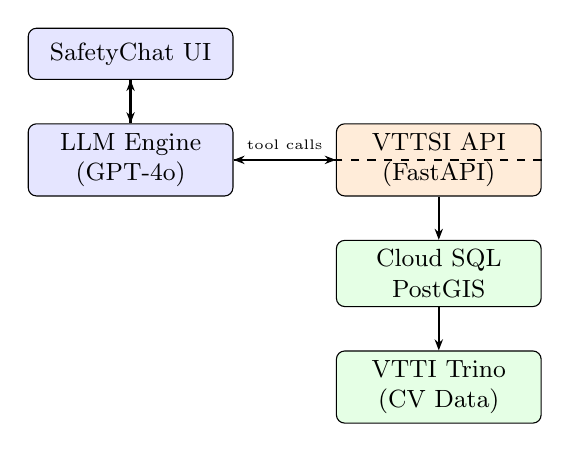
\begin{tikzpicture}[
        node distance = 0.55cm and 0.9cm,
        box/.style = {rectangle, draw, rounded corners=3pt,
                      minimum width=2.6cm, minimum height=0.65cm,
                      text centered, align=center, font=\small},
        llm/.style = {box, fill=blue!10},
        api/.style = {box, fill=orange!15},
        db/.style  = {box, fill=green!10},
        arr/.style = {-{Stealth[length=4pt]}, thick}
    ]
    \node[llm] (ui)      {SafetyChat UI};
    \node[llm, below=of ui] (llm)  {LLM Engine\\(GPT-4o)};
    \node[api, right=of llm, xshift=0.4cm] (api)  {VTTSI API\\(FastAPI)};
    \node[db,  below=of api] (db)   {Cloud SQL\\PostGIS};
    \node[db,  below=of db]  (trino){VTTI Trino\\(CV Data)};
    \draw[arr] (ui)  -- (llm);
    \draw[arr] (llm) -- node[above,font=\tiny]{tool calls} (api);
    \draw[arr] (api) -- (db);
    \draw[arr] (db)  -- (trino);
    \draw[arr,dashed] (api) -- ++(1.0,0) |- (llm);
    \draw[arr,dashed] (llm) -- (ui);
    \end{tikzpicture}
    \caption{SafetyChat data flow. Solid arrows: request path. Dashed: response path.}
    \label{fig:safetychat-flow}
\end{figure}

\subsection{Design Rationale}

VTTSI already answers \emph{what} the safety score is; SafetyChat answers \emph{why}
and \emph{what to do}.
We adopt a \emph{tool-augmented} LLM pattern \cite{toolformer2023}: the language model
is equipped with a small set of typed function calls that map to VTTSI REST endpoints,
so all numerical claims in the generated narrative are grounded in live API data rather
than model hallucination.

\subsection{LLM Tool Definitions}

SafetyChat exposes four tools to the LLM via the OpenAI function-calling protocol
\cite{openai_functioncalling}:

\begin{enumerate}
    \item \texttt{get\_safety\_score(intersection, window)} ---
          returns current RT--SI, MCDM, and blended scores with top contributing factors.
    \item \texttt{get\_component\_breakdown(intersection, time)} ---
          returns the weighted criterion values (vehicle count, VRU count, avg speed,
          speed variance, incident count) and CRITIC weights for the requested bin.
    \item \texttt{get\_historical\_baseline(intersection)} ---
          returns the EB prior, 7-year crash severity breakdown, and $\lambda^\star$.
    \item \texttt{compare\_intersections(intersection\_list, metric)} ---
          ranks a list of intersections by any index component over a lookback window.
\end{enumerate}

The system prompt instructs the LLM to cite tool outputs explicitly (e.g., quoting
numerical values), avoid extrapolating beyond available data, and flag data-gap periods
when telemetry is sparse.

\subsection{Differentiation from Existing Systems}

Table~\ref{tbl:comparison} summarizes how VTTSI-Chat differs from related systems.
Existing LLM+traffic systems target either \emph{signal control}
\cite{llmlight2024,trafficgpt2023} or \emph{AV motion planning}
\cite{gptdriver2023,drivevlm2024}; none operate on a hybrid crash--telemetry safety
index to generate operator-facing safety narratives.
Commercial safety dashboards (e.g., StreetLight, Waycare) provide ML predictions with no
conversational or causal explanation layer.

\begin{table}[t]
\centering
\caption{VTTSI-Chat vs.\ Related Systems}
\label{tbl:comparison}
\small
\begin{tabularx}{\columnwidth}{@{}l c c c c@{}}
\toprule
\textbf{System} & \textbf{\shortstack{Hybrid\\Safety\\Index}} &
\textbf{\shortstack{Real-Time\\Telemetry}} &
\textbf{\shortstack{LLM\\Interface}} &
\textbf{\shortstack{Causal\\Narrative}} \\
\midrule
Google Maps / Apple Maps  & \xmark & \cmark & \xmark & \xmark \\
Waycare (commercial)      & \xmark & \cmark & \xmark & \xmark \\
ATSPM (FHWA)              & \xmark & \cmark & \xmark & \xmark \\
TrafficGPT \cite{trafficgpt2023} & \xmark & \cmark & \cmark & \xmark \\
LLMLight \cite{llmlight2024}     & \xmark & \cmark & \cmark & \xmark \\
GPT-Driver \cite{gptdriver2023}  & \xmark & \cmark & \cmark & \xmark \\
\textbf{VTTSI-Chat (ours)}       & \cmark & \cmark & \cmark & \cmark \\
\bottomrule
\end{tabularx}
\end{table}

% ─────────────────────────────────────────────────────────
\section{Demo Scenarios and Use Cases}
\label{sec:demo}

The live demonstration runs against the production VTTSI deployment
(\url{https://cs6604-trafficsafety-180117512369.europe-west1.run.app/}) and a
co-deployed SafetyChat service.
Attendees interact directly with the chat interface.
Four primary use cases are shown.

\subsection{Use Case 1: TMC Operator Morning Briefing}

\textit{Scenario:} A TMC operator asks: \emph{``Give me a morning safety briefing
for all monitored intersections.''} \\
\textit{Demo Action:} SafetyChat calls \texttt{compare\_intersections} to rank all
intersections by blended score, then \texttt{get\_component\_breakdown} for the two
highest-ranked sites. It produces a narrative identifying peak-hour risk windows,
dominant driving factors (e.g., speed variance spike, elevated VRU counts), and
compares scores to the 7-day rolling average.

\textit{Distinction:} The existing Streamlit dashboard requires the operator to
navigate multiple charts; SafetyChat synthesizes multi-intersection data into a
single situational-awareness paragraph in under five seconds.

\subsection{Use Case 2: Causal Safety Explanation for Planners}

\textit{Scenario:} A transportation planner asks: \emph{``Why did the
E.~Broad--N.~Washington intersection score above 70 yesterday at 5\,PM?''} \\
\textit{Demo Action:} SafetyChat retrieves the 15-minute bin data, identifies that
both vehicle count and incident count were in the 90th percentile, and notes that
CRITIC assigned elevated weight to incident count in that period. The narrative
explains that a cluster of red-light-running events co-occurred with peak through-volume,
consistent with the intersection's historical risk profile from VDOT crash records.

\subsection{Use Case 3: Emergency Responder Routing Support}

\textit{Scenario:} An emergency dispatcher asks: \emph{``Which intersection between
Glebe--Potomac and Birch--W.~Broad has lower current risk for a priority vehicle
crossing?''} \\
\textit{Demo Action:} SafetyChat calls \texttt{get\_safety\_score} for both
intersections, comparing RT--SI, MCDM, and blended indices in real time, and identifies
the lower-risk option with reasoning grounded in current VRU counts and speed variance.

\subsection{Use Case 4: Public or Stakeholder Engagement}

\textit{Scenario:} A city council member, unfamiliar with transportation engineering,
asks: \emph{``Is my neighborhood intersection getting safer over time?''} \\
\textit{Demo Action:} SafetyChat retrieves the 30-day trend from the blended index
and, where available, contextualizes it against VDOT crash severity trends, translating
index values into plain-language risk levels (e.g., ``The score has dropped from 45 to
31 over the past month, meaning current conditions are \emph{moderate risk},
comparable to early-morning weekend conditions'').

\begin{table}[t]
\centering
\caption{Summary of Demo Use Cases}
\label{tbl:usecases}
\small
\begin{tabularx}{\columnwidth}{@{}l X l@{}}
\toprule
\textbf{Use Case} & \textbf{Key Interaction} & \textbf{Primary User} \\
\midrule
Morning briefing        & Multi-intersection rank + narrative         & TMC Operator \\
Causal explanation      & Score decomposition, CRITIC weight trace    & Planner \\
Responder routing       & Comparative real-time score query           & Dispatcher \\
Public engagement       & Trend + plain-language risk translation     & Official / Public \\
\bottomrule
\end{tabularx}
\end{table}

% ─────────────────────────────────────────────────────────
\section{Related Work}
\label{sec:related}

\textbf{Crash-based and hybrid safety indices.}
EB-stabilized crash models \cite{persaud2007,montella2020systemic} and MCDM-based
indices \cite{Amraji2025CombinedSafetyIndex,asadamraji2025combined} provide the
theoretical foundation for VTTSI's scoring pipeline. Surrogate safety indicators
\cite{schultz2025_surrogate,gettman2003ssam} complement crash data with real-time
conflict proxies. VTTSI unifies these streams; the SafetyChat module adds the
explanation layer that prior hybrid-index systems lack.

\textbf{LLMs in transportation.}
TrafficGPT \cite{trafficgpt2023} applies GPT-class models to traffic flow analysis and
signal timing; it does not provide a safety index or causal narrative.
LLMLight \cite{llmlight2024} uses LLMs as traffic signal controllers via reinforcement
learning prompts; it is limited to signal optimization.
GPT-Driver \cite{gptdriver2023} and DriveVLM \cite{drivevlm2024} apply LLMs to
vehicle-level motion planning; they operate at the AV layer, not the infrastructure
monitoring layer.
Behboudi et al.\ \cite{Behboudi2024} survey ML-based crash analysis but do not address
conversational interfaces or real-time hybrid indices.

\textbf{Positioning.}
VTTSI-Chat is differentiated by combining: (i) a \emph{validated hybrid safety index}
that fuses long-term crash history with 15-minute telemetry, (ii) a
\emph{tool-augmented LLM} that accesses live API data rather than relying on embedded
knowledge, and (iii) operator-facing \emph{causal narratives} that trace score
components back to raw signals. No existing system offers all three.

% ─────────────────────────────────────────────────────────
\section{Conclusion}
\label{sec:conclusion}

This demo presents VTTSI-Chat, a cloud-native intersection safety system that pairs a
hybrid EB + MCDM safety index with a tool-augmented LLM frontend.
The SafetyChat module closes the gap between quantitative safety scores and
human-readable, causally grounded situational awareness, enabling TMC operators,
planners, emergency responders, and the public to engage with real-time safety
intelligence through natural language.
By grounding all LLM outputs in live API calls, SafetyChat avoids hallucination while
retaining the flexibility of conversational interaction.
Future work will integrate the Agentic Traffic Safety Knowledge Graph (TS--KG)
\cite{cusati2025agentickg} as an additional tool, enabling the LLM to reason over
intersection geometry, conflict topology, and causal trajectory motifs.

\section*{Acknowledgment}
This research used AI assistance in generating content. The VTTSI system was developed
in collaboration with the Virginia Tech Transportation Institute (VTTI).

\printbibliography

\end{document}
